\documentclass{article}

\usepackage{../../common/labconfig}
\usepackage{../../common/labstyle}

\usepackage{tikz-timing}[2014/10/29]
\usetikztiminglibrary[rising arrows]{clockarrows}
\usepackage{xparse} % NewDocumentCommand, IfValueTF, IFBooleanTF

\NewDocumentCommand{\busref}{som}{\texttt{%
		#3%
		\IfValueTF{#2}{[#2]}{}%
		\IfBooleanTF{#1}{\#}{}%
}}

\lhead{Virtual I2C Lab (Master and Slave)}

\begin{document}

\section{Introduction}

The objective of this lab is to read sensor data conveyed by a sensor
(VD-004) to your simulated CPU using I2C master write transactions.
Your simulated CPU will store each sensor value to a storage device
(VD-005) using I2C master write operations.

This lab will use a ``bit-banged'' implementation of the I2C protocol.

\begin{figure}[H]

	\centering

	\begin{tabular}{r|l}

		Part & Due Date \\ \hline\hline
		Code & Apr. 28\\

	\end{tabular}

	\caption{Table of due dates for each part.}

\end{figure}

\tableofcontents

\section{How to Submit }

When your code is ready to turn in, please submit only your \texttt{main.cpp}
file via Moodle. Note that you should write all code that you need within
\texttt{main.cpp}. As before, your code must compile to receive any credit.

\section{Simulated Devices}

In this lab, you will interface with two virtual devices using I2C, a sensor
and a flash memory.

Normally, all three devices should share common \texttt{scl} and \texttt{sda}
lines, as shown below.

\begin{figure}[H]
	\centering
       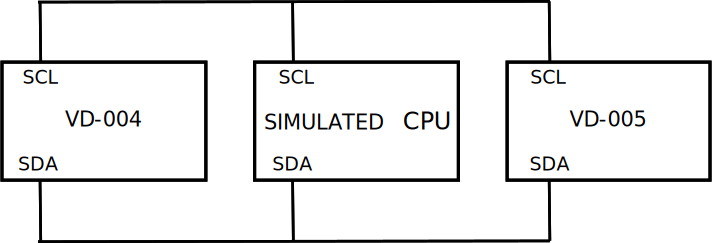
\includegraphics[max width = 0.7\textwidth]{i2c_base.pdf}
	\caption{Topology of the simulated devices.}
\end{figure}

However, due to limitations of software emulation using Verilator, we
adopt a slightly different approach, where the values of \texttt{scl} and
\texttt{sda} will be automatically selected from the values of \texttt{scl}
and \texttt{sda} being driven from each of the three devices.  Only one device controls each line at one time.

This is relevant when viewing the waves generated from
your code, in which you'll see traces for \texttt{sda}, \texttt{sda\_i},
\texttt{scl}, and \texttt{scl\_i}.  The values for \texttt{sda} and
\texttt{sda\_i} will always be identical except during periods when VD-004
or VD-005 is actively driving the wire (the same applies to \texttt{scl} and
\texttt{scl\_i}).  Note that you will still read and write to \texttt{IO\_SDA}
and \texttt{IO\_SCL} and you don't need to do anything special to ``yield''
control of either line to one of the peripherals (they will claim these lines
whenever needed).

\begin{figure}[H]
	\centering
	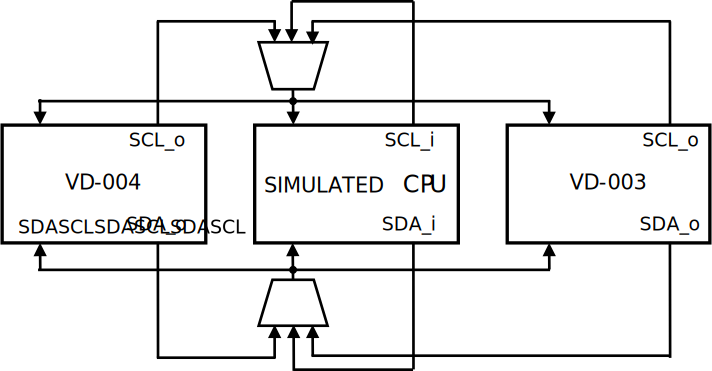
\includegraphics[max width = 0.7\textwidth]{i2c_uni.pdf}
	\caption{Topology of the simulated devices.}
\end{figure}

\subsection{VD-004: Simulated Sensor}

\textbf{Read this section carefully as it has changed since the previous lab.}

The VD-004 collects sensor readings that may contain between 1 and 128 bytes of
data.  It will begin collecting data once your design reads the NPAGE register from
VD-005 (see below).  After this, VD-004 will perform an I2C master write operations
to the simulated CPU after every 200 clock cycles of idle time.

When VD-004 is ready to send a batch of sensor values, it will send $n+1$ write
transactions to the simulated CPU.  The first of these will contain the number
of sensor readings to follow.  The next $n$ transactions will contain the sensor
values.  Afterward it will repeat this sequence.

The I2C address of your simulated CPU is 0x7A.  Your simulated CPU should only
repond to the master write request if the requested address is correct.

\subsection{VD-005: Simulated Flash Memory}

The VD-005 simulates a flash memory storage device. In this lab it will use a
simplified interface, in which consecutive writes to the DATA register will automatically
be placed into consecutive locations on the selected page.  This way, your code will
no longer need to write the OFFSET register.  Also, you no longer need to write the
magic number.

The register map for VD-005 is shown in the table below.

\begin{figure}[H]

	\centering

	\begin{tabular}{c | c | c | p{0.5\textwidth}}

		Register Address & Name & Mode(s) & Description \\ \hline\hline

		\texttt{0x1D} & \texttt{NPAGE} & read & Returns the number of pages on the flash device. \\ \hline

		\texttt{0x1B} & \texttt{PAGESEL} & write & Selects which page of memory to write. \\ \hline

		\texttt{0x1C} & \texttt{WHO\_AM\_I} & read & Always contains the value \texttt{0x36} \\ \hline

		\texttt{0x1F} & \texttt{DATA} & write & Specifies the value at the active address on the active page. \\


	\end{tabular}

	\caption{Table of VD-005 registers.}

\end{figure}

\subsection{Program Requirements}

Your program should first query the \texttt{WHO\_AM\_I} on VD-005 and verify it
returns the correct value. If not, then your program should display an error
message (on standard out) and exit.

Your program should also query the \texttt{NPAGE} register of the VD-005 to
determine the number of pages of memory available.  Note that reading this
register will cause VD-004 to begin performing I2C master write transactions
after every 200 cycles of idle time.

Finally, your program should enter an infinite loop, waiting for an I2C master
write from VD-004 containing the number of sensor readings, writing the page
number to VD-005, then alternating between waiting for each new sensor reading
from VD-004 and writing it to VD-005.

This will give way to the following sequence:
\begin{itemize}
	
	\item read VD-005.WHO\_AM\_I
	\item read VD-005.NPAGE
	\item receive VD-004.NREADINGS
	\item write VD-004.PAGESEL
	\item receive VD-004.D0 (first sensor byte)
	\item write VD-004.DATA	
	\item receive VD-004.D1 (second sensor byte)
	\item write VD-004.DATA	
	\item ...
	\item receive VD-004.Dn (nth sensor byte)
	\item write VD-004.DATA
	\item receive VD-004.NREADINGS
	\item write VD-004.PAGESEL
	\item receive VD-004.D0 (first sensor byte)
	\item write VD-004.DATA	
	\item receive VD-004.D1 (second sensor byte)
	\item write VD-004.DATA
	\item ...
	
\end{itemize}

Once your program has exhausted the available supply of flash memory pages (the
number of pages available can be determined by the \texttt{NPAGE} register of
the VD-005), it should exit with an informative message indicating no further
flash memory is available.

\section{Programming Environment}

The programming environment for this lab is very different from the
previous lab.  There only two pins: \texttt{IO\_SDA} and \texttt{IO\_SCL}, which
may be read with \texttt{read\_io()} or written with \texttt{write\_io()}.

You do not need to implement recovery from NACK (not-acknowledge) flags in
I2C transactions.

\section{Provided Code}

We will provide you with the following functions and macros:
\begin{itemize}
\item the \texttt{main()} function
\item the \texttt{master\_i2c()} function, which performs a master read or write operation (use this to
communicate with VD-005),
\item the \texttt{WAIT\_FOR\_START\_BIT()} macro, which will advance the simulation until an I2C start bit
is seen; after this macro returns, expect the simulation time to be one simulation cycle past the falling edge
of SDA,
\item the \texttt{WAIT\_FOR\_STOP\_BIT()} macro, which will advance the simulation until an I2C stop bit
is seen; after this macro returns, expect the simulation time to be one simulation cycle past the rising edge
of SDA,
\item the \texttt{WAIT\_FOR\_RISING\_SCL()} macro, which will advance the simulation until the next rising
edge of SCL; after this macro returns, expect the simulation time to be one simulation cycle past the rising edge
of SCL, and
\item the \texttt{WAIT\_FOR\_FALLING\_SCL()} macro, which will advance the simulation until the next falling
edge of SCL; after this macro returns, expect the simulation time to be one simulation cycle past the falling edge
of SCL.
\end{itemize}

\section{Suggested Plan of Work}

We suggest you follow these steps:
\begin{enumerate}
	\item Read the comments in the code, including the placeholders in the \texttt{slave\_i2c()} function
	\item Fill in the missing code in the \texttt{slave\_i2c()} function
	\item As with Lab 2 and Lab 3, test your code with ``make simulation \&\& ./simulation,''  ``make waves,''
		``make decode,'' and ``make flashdump''.
\end{enumerate}

\section{Grading}

Your code will be inspected for style and correctness by a human reader. This
aspect of grading will be fairly lenient and mostly for the purpose of giving
you useful feedback. However you may still lose points for egregious stylistic
problems, or failing to write code that clearly attempts to solve the problem
at hand.

Your code will also be run against the same simulated sensor as you are given
in the project skeleton, however the hard-coded sensor "readings" will be
changed to different values. \textbf{The length of sensor data streams and the
number of flash memory pages will also be changed during grading, so make sure
your program accounts for this.}

Additionally, your code will be run against a version of the simulated sensor
and/or flash memory which is defective, and reports an incorrect value when the
\texttt{WHO\_AM\_I} register is read. In such cases, your program should exit
with an informative error message. \textbf{You may assume that if a VD-004 or
VD-005 reports a correct \texttt{WHO\_AM\_I} value, it is not defective.}

The correctness of your code will primarily judged by evaluating the output of
\texttt{make flashdump} using an alternate set of sensor data, however any
printouts your code displays, as well as the output of sigrok via \texttt{make
decode} may be used as a supplement.

If your code does not compile and run on the CSCE linux lab computers, you will
not receive credit.

\section{Rubric}

\begin{itemize}

	\item 10 points - Code style

	\item 10 points - Correct checking of \texttt{WHO\_AM\_I} register

	\item 10 points - Data is read via I2C master writes from the sensor.

	\item 10 points - Data is stored in the VD-005 in the proper format.

	\item 10 points - Data stored in the VD-005 is correct/matches the
		hard-coded values from the sensor (format must also be
		correct).

	\item $\frac{5}{2} \times b$ points - See "Bug Bounty".

\end{itemize}

\textbf{Maximum number of points possible: 50.}

Keep in mind that some items not listed on the rubric may cause you to loose
points, including cheating, submitting code which is inconsistent with what you
have demonstrating, plagiarizing code or reflection content, etc.

\section{Bug Bounty (Extra Credit Opportunity)}

There is an extra credit opportunity available for this lab. If you find a bug
in our code, we will increment the $b$ counter in the rubric above once for
each bug. In other words, you will earn 2.5 bonus points per bug. If this puts
your grade on this project higher than 50 points, you will receive $b$ many
bonus points on the final exam (i.e. each bug you find will improve your final
exam score by 1\%).

To take advantage of this opportunity, you must send us an email with the
following example:

\begin{itemize}

	\item A zipped up copy of your code.

	\item A clear description of the bug and how to re-produce it.

	\item A clear description of how the bug causes the code to behave in a
		manner inconsistent with what is documented in this lab sheet,
		or in a fashion that is otherwise problematic.

\end{itemize}

If your bug stems from your own code, or a mis-understanding of the course
material, you will neither gain nor lose points ($b$ remains unchanged).
However submitting a bug report without all three of the items above will
result in $b$ being decremented, and possibly becoming negative as a result.

Minor typos, compiler warnings, etc. do not count as bugs, but please feel
welcome to report them if you find them.

If multiple students discover the same bug, they will all receive the bonus.
However, reports emailed after a fix has been announced or otherwise
distributed to the class are not eligible to receive the extra credit. To
receive the bonus, your bug report must be submitted no later than Monday,
April 27, 2020 at midnight eastern time.

\end{document}
